%!TEX root = ../thesis.tex

\thispagestyle{myheadings}

\graphicspath{{Body/Figures/Wa/Datasets/Endgame/SingleIteration/CaloFits/}{Body/Figures/Wa/Datasets/60h/SingleIteration/SingleFits/}{Body/Figures/Wa/Datasets/HighKick/SingleIteration/SingleFits/}{Body/Figures/Wa/Datasets/9d/SingleIteration/SingleFits/}{Body/Figures/Wa/Datasets/Endgame/SingleIteration/SingleFits/}}


\chapter{Fit Result Correlation Matrices}
\label{app:CorrelationMatrices}

Correlation matrices for the 60h, HighKick, 9d, and Endgame datasets. It was found that there were stronger correlations between higher order CBO parameters in the HighKick and 9d datasets than in the 60h and Endgame datasets.


\begin{figure}
    \centering
    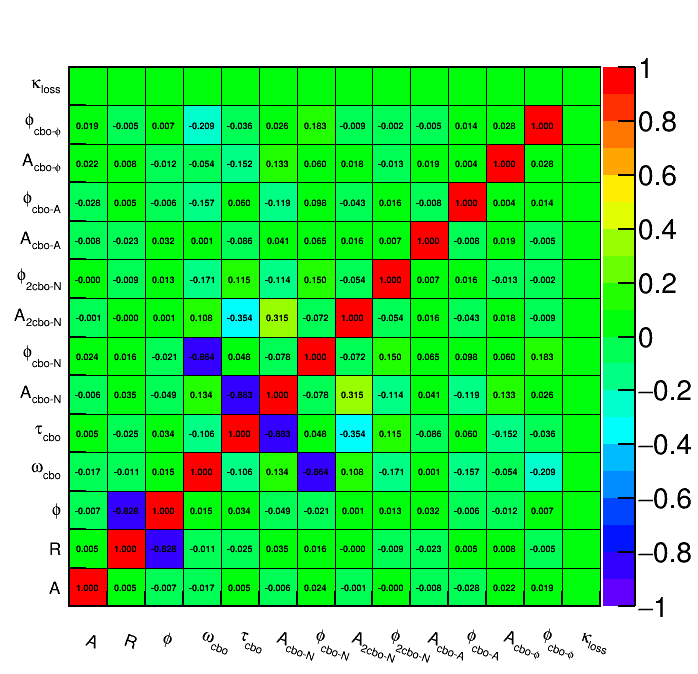
\includegraphics[width=\textwidth]{CorrelationMatrixFullRatioFit_60h}
    \caption[60h ratio fit correlation matrix]{Correlation matrix for a single seed ratio fit to the 60h dataset. The only significant correlation with $R$ is the \gmtwo phase. \K is fixed, hence the corresponding empty row and column.}
    \label{fig:CorrMat_60h}
\end{figure}


\begin{figure}
    \centering
    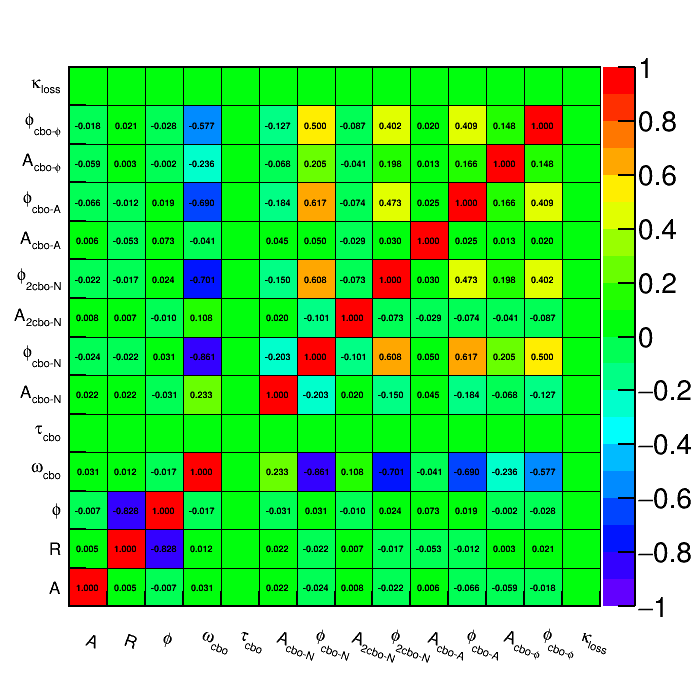
\includegraphics[width=\textwidth]{CorrelationMatrixFullRatioFit_HighKick}
    \caption[HighKick ratio fit correlation matrix]{Correlation matrix for the single seed ratio fit to the HighKick dataset. The only significant correlation with $R$ is the \gmtwo phase. $\tau_{cbo}$ and \K are fixed, hence the corresponding empty rows and columns.}
    \label{fig:CorrMat_HighKick}
\end{figure}

\begin{figure}
    \centering
    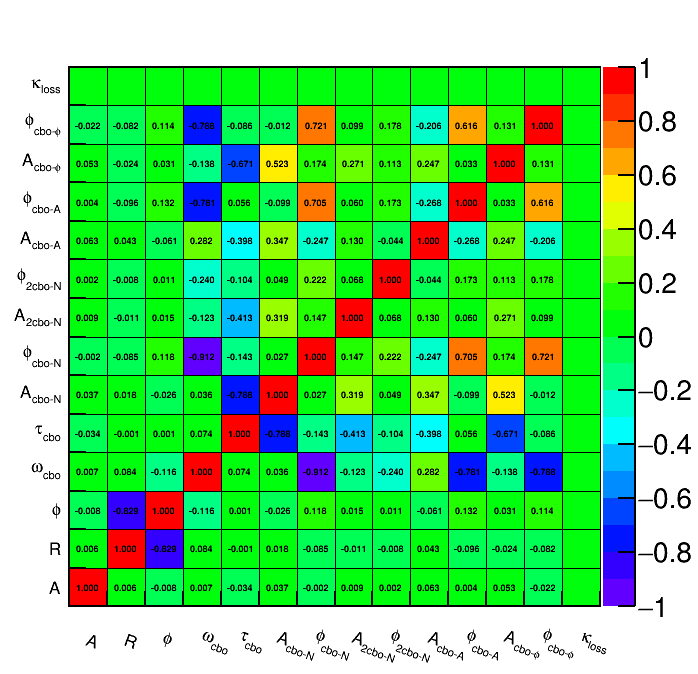
\includegraphics[width=\textwidth]{CorrelationMatrixFullRatioFit_9d}
    \caption[9d ratio fit correlation matrix]{Correlation matrix for the single seed ratio fit to the 9d dataset. The only significant correlation with $R$ is the \gmtwo phase. \K is fixed, hence the corresponding empty row and column.}
    \label{fig:CorrMat_9d}
\end{figure}


\begin{figure}
    \centering
    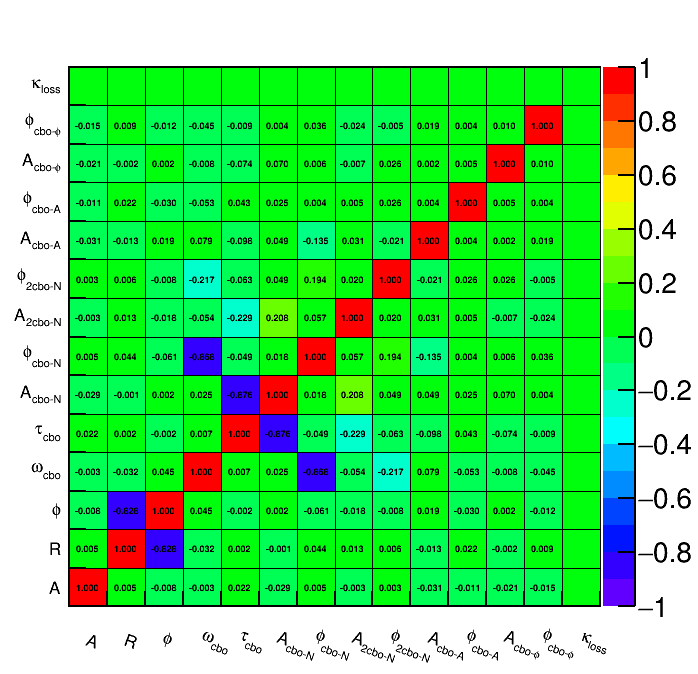
\includegraphics[width=\textwidth]{CorrelationMatrixFullRatioFit_Endgame}
    \caption[Endgame ratio fit correlation matrix]{Correlation matrix for the single seed ratio fit to the Endgame dataset. The only significant correlation with $R$ is the \gmtwo phase. \K is fixed, hence the corresponding empty row and column.}
    \label{fig:CorrMat_Endgame}
\end{figure}


% \begin{landscape}
% \begin{table}[]
% \setlength\tabcolsep{5pt}
% \footnotesize
% \begin{tabular*}{\linewidth}{@{\extracolsep{\fill}}lLBLLLLLLLLLLLL}
%   \toprule
%             & \thead{$A$} & \thead{$R$} & \thead{$\phi$} & \thead{$\omega_{cbo}$} & \thead{$\tau_{cbo}$} & \thead{$A_{cbo-N}$} & \thead{$\phi_{cbo-N}$} & \thead{$A_{2cbo-N}$} & \thead{$\phi_{2cbo-N}$} & \thead{$A_{cbo-A}$} & \thead{$\phi_{cbo-A}$} & \thead{$A_{cbo-\phi}$} & \thead{$\phi_{cbo-\phi}$} & \thead{$\kappa_{loss}$} \\
%   \midrule
% $A$                & 1.000 & 0.005 & -0.007 & -0.017 & 0.005 & -0.006 & 0.024 & -0.001 & -0.000 & -0.008 & -0.028 & 0.022 & 0.019 & 0.000  \\
% $R$                & 0.005 & 1.000 & -0.828 & -0.011 & -0.025 & 0.035 & 0.016 & -0.000 & -0.009 & -0.023 & 0.005 & 0.008 & -0.005 & 0.000  \\
% $\phi$             & -0.007 & -0.828 & 1.000 & 0.015 & 0.034 & -0.049 & -0.021 & 0.001 & 0.013 & 0.032 & -0.006 & -0.012 & 0.007 & 0.000  \\
% $\omega_{cbo}$     & -0.017 & -0.011 & 0.015 & 1.000 & -0.106 & 0.134 & -0.864 & 0.108 & -0.171 & 0.001 & -0.157 & -0.054 & -0.209 & 0.000  \\
% $\tau_{cbo}$       & 0.005 & -0.025 & 0.034 & -0.106 & 1.000 & -0.883 & 0.048 & -0.354 & 0.115 & -0.086 & 0.060 & -0.152 & -0.036 & 0.000  \\
% $A_{cbo-N}$        & -0.006 & 0.035 & -0.049 & 0.134 & -0.883 & 1.000 & -0.078 & 0.315 & -0.114 & 0.041 & -0.119 & 0.133 & 0.026 & 0.000  \\
% $\phi_{cbo-N}$     & 0.024 & 0.016 & -0.021 & -0.864 & 0.048 & -0.078 & 1.000 & -0.072 & 0.150 & 0.065 & 0.098 & 0.060 & 0.183 & 0.000  \\
% $A_{2cbo-N}$       & -0.001 & -0.000 & 0.001 & 0.108 & -0.354 & 0.315 & -0.072 & 1.000 & -0.054 & 0.016 & -0.043 & 0.018 & -0.009 & 0.000  \\
% $\phi_{2cbo-N}$    & -0.000 & -0.009 & 0.013 & -0.171 & 0.115 & -0.114 & 0.150 & -0.054 & 1.000 & 0.007 & 0.016 & -0.013 & -0.002 & 0.000  \\
% $A_{cbo-A}$        & -0.008 & -0.023 & 0.032 & 0.001 & -0.086 & 0.041 & 0.065 & 0.016 & 0.007 & 1.000 & -0.008 & 0.019 & -0.005 & 0.000  \\
% $\phi_{cbo-A}$     & -0.028 & 0.005 & -0.006 & -0.157 & 0.060 & -0.119 & 0.098 & -0.043 & 0.016 & -0.008 & 1.000 & 0.004 & 0.014 & 0.000  \\
% $A_{cbo-\phi}$     & 0.022 & 0.008 & -0.012 & -0.054 & -0.152 & 0.133 & 0.060 & 0.018 & -0.013 & 0.019 & 0.004 & 1.000 & 0.028 & 0.000  \\
% $\phi_{cbo-\phi}$  & 0.019 & -0.005 & 0.007 & -0.209 & -0.036 & 0.026 & 0.183 & -0.009 & -0.002 & -0.005 & 0.014 & 0.028 & 1.000 & 0.000  \\
% $\kappa_{loss}$    & 0.000 & 0.000 & 0.000 & 0.000 & 0.000 & 0.000 & 0.000 & 0.000 & 0.000 & 0.000 & 0.000 & 0.000 & 0.000 & 0.000  \\
%   \bottomrule
% \end{tabular*}
% \caption[60h ratio fit correlation matrix]{Correlation matrix for the ratio fit to the 60h dataset.}
% \label{Tab:CorrMat_60h}
% \end{table}
% \end{landscape}



% \begin{landscape}
% \begin{table}[]
% \setlength\tabcolsep{5pt}
% \footnotesize
% \begin{tabular*}{\linewidth}{@{\extracolsep{\fill}}lLBLLLLLLLLLLLL}
%   \toprule
%             & \thead{$A$} & \thead{$R$} & \thead{$\phi$} & \thead{$\omega_{cbo}$} & \thead{$\tau_{cbo}$} & \thead{$A_{cbo-N}$} & \thead{$\phi_{cbo-N}$} & \thead{$A_{2cbo-N}$} & \thead{$\phi_{2cbo-N}$} & \thead{$A_{cbo-A}$} & \thead{$\phi_{cbo-A}$} & \thead{$A_{cbo-\phi}$} & \thead{$\phi_{cbo-\phi}$} & \thead{$\kappa_{loss}$} \\
%   \midrule
% $A$                & 1.000 & 0.005 & -0.007 & 0.031 & 0.000 & 0.022 & -0.024 & 0.008 & -0.022 & 0.006 & -0.066 & -0.059 & -0.018 & 0.000  \\
% $R$                & 0.005 & 1.000 & -0.828 & 0.012 & 0.000 & 0.022 & -0.022 & 0.007 & -0.017 & -0.053 & -0.012 & 0.003 & 0.021 & 0.000  \\
% $\phi$             & -0.007 & -0.828 & 1.000 & -0.017 & 0.000 & -0.031 & 0.031 & -0.010 & 0.024 & 0.073 & 0.019 & -0.002 & -0.028 & 0.000  \\
% $\omega_{cbo}$     & 0.031 & 0.012 & -0.017 & 1.000 & 0.000 & 0.233 & -0.861 & 0.108 & -0.701 & -0.041 & -0.690 & -0.236 & -0.577 & 0.000  \\
% $\tau_{cbo}$       & 0.000 & 0.000 & 0.000 & 0.000 & 0.000 & 0.000 & 0.000 & 0.000 & 0.000 & 0.000 & 0.000 & 0.000 & 0.000 & 0.000  \\
% $A_{cbo-N}$        & 0.022 & 0.022 & -0.031 & 0.233 & 0.000 & 1.000 & -0.203 & 0.020 & -0.150 & 0.045 & -0.184 & -0.068 & -0.127 & 0.000  \\
% $\phi_{cbo-N}$     & -0.024 & -0.022 & 0.031 & -0.861 & 0.000 & -0.203 & 1.000 & -0.101 & 0.608 & 0.050 & 0.617 & 0.205 & 0.500 & 0.000  \\
% $A_{2cbo-N}$       & 0.008 & 0.007 & -0.010 & 0.108 & 0.000 & 0.020 & -0.101 & 1.000 & -0.073 & -0.029 & -0.074 & -0.041 & -0.087 & 0.000  \\
% $\phi_{2cbo-N}$    & -0.022 & -0.017 & 0.024 & -0.701 & 0.000 & -0.150 & 0.608 & -0.073 & 1.000 & 0.030 & 0.473 & 0.198 & 0.402 & 0.000  \\
% $A_{cbo-A}$        & 0.006 & -0.053 & 0.073 & -0.041 & 0.000 & 0.045 & 0.050 & -0.029 & 0.030 & 1.000 & 0.025 & 0.013 & 0.020 & 0.000  \\
% $\phi_{cbo-A}$     & -0.066 & -0.012 & 0.019 & -0.690 & 0.000 & -0.184 & 0.617 & -0.074 & 0.473 & 0.025 & 1.000 & 0.166 & 0.409 & 0.000  \\
% $A_{cbo-\phi}$     & -0.059 & 0.003 & -0.002 & -0.236 & 0.000 & -0.068 & 0.205 & -0.041 & 0.198 & 0.013 & 0.166 & 1.000 & 0.148 & 0.000  \\
% $\phi_{cbo-\phi}$  & -0.018 & 0.021 & -0.028 & -0.577 & 0.000 & -0.127 & 0.500 & -0.087 & 0.402 & 0.020 & 0.409 & 0.148 & 1.000 & 0.000  \\
% $\kappa_{loss}$    & 0.000 & 0.000 & 0.000 & 0.000 & 0.000 & 0.000 & 0.000 & 0.000 & 0.000 & 0.000 & 0.000 & 0.000 & 0.000 & 0.000  \\
%   \bottomrule
% \end{tabular*}
% \caption[HighKick ratio fit correlation matrix]{Correlation matrix for the ratio fit to the HighKick dataset.}
% \label{Tab:CorrMat_HighKick}
% \end{table}
% \end{landscape}






% \begin{landscape}
% \begin{table}[]
% \setlength\tabcolsep{5pt}
% \footnotesize
% \begin{tabular*}{\linewidth}{@{\extracolsep{\fill}}lLBLLLLLLLLLLLL}
%   \toprule
%             & \thead{$A$} & \thead{$R$} & \thead{$\phi$} & \thead{$\omega_{cbo}$} & \thead{$\tau_{cbo}$} & \thead{$A_{cbo-N}$} & \thead{$\phi_{cbo-N}$} & \thead{$A_{2cbo-N}$} & \thead{$\phi_{2cbo-N}$} & \thead{$A_{cbo-A}$} & \thead{$\phi_{cbo-A}$} & \thead{$A_{cbo-\phi}$} & \thead{$\phi_{cbo-\phi}$} & \thead{$\kappa_{loss}$} \\
%   \midrule
% $A$                & 1.000 & 0.006 & -0.008 & 0.007 & -0.034 & 0.037 & -0.002 & 0.009 & 0.002 & 0.063 & 0.004 & 0.053 & -0.022 & 0.000  \\
% $R$                & 0.006 & 1.000 & -0.829 & 0.084 & -0.001 & 0.018 & -0.085 & -0.011 & -0.008 & 0.043 & -0.096 & -0.024 & -0.082 & 0.000  \\
% $\phi$             & -0.008 & -0.829 & 1.000 & -0.116 & 0.001 & -0.026 & 0.118 & 0.015 & 0.011 & -0.061 & 0.132 & 0.031 & 0.114 & 0.000  \\
% $\omega_{cbo}$     & 0.007 & 0.084 & -0.116 & 1.000 & 0.074 & 0.036 & -0.912 & -0.123 & -0.240 & 0.282 & -0.781 & -0.138 & -0.788 & 0.000  \\
% $\tau_{cbo}$       & -0.034 & -0.001 & 0.001 & 0.074 & 1.000 & -0.788 & -0.143 & -0.413 & -0.104 & -0.398 & 0.056 & -0.671 & -0.086 & 0.000  \\
% $A_{cbo-N}$        & 0.037 & 0.018 & -0.026 & 0.036 & -0.788 & 1.000 & 0.027 & 0.319 & 0.049 & 0.347 & -0.099 & 0.523 & -0.012 & 0.000  \\
% $\phi_{cbo-N}$     & -0.002 & -0.085 & 0.118 & -0.912 & -0.143 & 0.027 & 1.000 & 0.147 & 0.222 & -0.247 & 0.705 & 0.174 & 0.721 & 0.000  \\
% $A_{2cbo-N}$       & 0.009 & -0.011 & 0.015 & -0.123 & -0.413 & 0.319 & 0.147 & 1.000 & 0.068 & 0.130 & 0.060 & 0.271 & 0.099 & 0.000  \\
% $\phi_{2cbo-N}$    & 0.002 & -0.008 & 0.011 & -0.240 & -0.104 & 0.049 & 0.222 & 0.068 & 1.000 & -0.044 & 0.173 & 0.113 & 0.178 & 0.000  \\
% $A_{cbo-A}$        & 0.063 & 0.043 & -0.061 & 0.282 & -0.398 & 0.347 & -0.247 & 0.130 & -0.044 & 1.000 & -0.268 & 0.247 & -0.206 & 0.000  \\
% $\phi_{cbo-A}$     & 0.004 & -0.096 & 0.132 & -0.781 & 0.056 & -0.099 & 0.705 & 0.060 & 0.173 & -0.268 & 1.000 & 0.033 & 0.616 & 0.000  \\
% $A_{cbo-\phi}$     & 0.053 & -0.024 & 0.031 & -0.138 & -0.671 & 0.523 & 0.174 & 0.271 & 0.113 & 0.247 & 0.033 & 1.000 & 0.131 & 0.000  \\
% $\phi_{cbo-\phi}$  & -0.022 & -0.082 & 0.114 & -0.788 & -0.086 & -0.012 & 0.721 & 0.099 & 0.178 & -0.206 & 0.616 & 0.131 & 1.000 & 0.000  \\
% $\kappa_{loss}$    & 0.000 & 0.000 & 0.000 & 0.000 & 0.000 & 0.000 & 0.000 & 0.000 & 0.000 & 0.000 & 0.000 & 0.000 & 0.000 & 0.000  \\
%   \bottomrule
% \end{tabular*}
% \caption[9d ratio fit correlation matrix]{Correlation matrix for the ratio fit to the 9d dataset.}
% \label{Tab:CorrMat_9d}
% \end{table}
% \end{landscape}



% \begin{landscape}
% \begin{table}[]
% \setlength\tabcolsep{5pt}
% \footnotesize
% \begin{tabular*}{\linewidth}{@{\extracolsep{\fill}}lLBLLLLLLLLLLLL}
%   \toprule
%             & \thead{$A$} & \thead{$R$} & \thead{$\phi$} & \thead{$\omega_{cbo}$} & \thead{$\tau_{cbo}$} & \thead{$A_{cbo-N}$} & \thead{$\phi_{cbo-N}$} & \thead{$A_{2cbo-N}$} & \thead{$\phi_{2cbo-N}$} & \thead{$A_{cbo-A}$} & \thead{$\phi_{cbo-A}$} & \thead{$A_{cbo-\phi}$} & \thead{$\phi_{cbo-\phi}$} & \thead{$\kappa_{loss}$} \\
%   \midrule
% $A$                & 1.000 & 0.005 & -0.008 & -0.003 & 0.022 & -0.029 & 0.005 & -0.003 & 0.003 & -0.031 & -0.011 & -0.021 & -0.015 & 0.000  \\
% $R$                & 0.005 & 1.000 & -0.828 & -0.032 & 0.002 & -0.001 & 0.044 & 0.013 & 0.006 & -0.013 & 0.022 & -0.002 & 0.009 & 0.000  \\
% $\phi$             & -0.008 & -0.828 & 1.000 & 0.045 & -0.002 & 0.002 & -0.061 & -0.018 & -0.008 & 0.019 & -0.030 & 0.002 & -0.012 & 0.000  \\
% $\omega_{cbo}$     & -0.003 & -0.032 & 0.045 & 1.000 & 0.007 & 0.025 & -0.868 & -0.054 & -0.217 & 0.079 & -0.053 & -0.008 & -0.045 & 0.000  \\
% $\tau_{cbo}$       & 0.022 & 0.002 & -0.002 & 0.007 & 1.000 & -0.876 & -0.049 & -0.229 & -0.063 & -0.098 & 0.043 & -0.074 & -0.009 & 0.000  \\
% $A_{cbo-N}$        & -0.029 & -0.001 & 0.002 & 0.025 & -0.876 & 1.000 & 0.018 & 0.208 & 0.049 & 0.049 & 0.025 & 0.070 & 0.004 & 0.000  \\
% $\phi_{cbo-N}$     & 0.005 & 0.044 & -0.061 & -0.868 & -0.049 & 0.018 & 1.000 & 0.057 & 0.194 & -0.135 & 0.004 & 0.006 & 0.036 & 0.000  \\
% $A_{2cbo-N}$       & -0.003 & 0.013 & -0.018 & -0.054 & -0.229 & 0.208 & 0.057 & 1.000 & 0.020 & 0.031 & 0.005 & -0.007 & -0.024 & 0.000  \\
% $\phi_{2cbo-N}$    & 0.003 & 0.006 & -0.008 & -0.217 & -0.063 & 0.049 & 0.194 & 0.020 & 1.000 & -0.021 & 0.026 & 0.026 & -0.005 & 0.000  \\
% $A_{cbo-A}$        & -0.031 & -0.013 & 0.019 & 0.079 & -0.098 & 0.049 & -0.135 & 0.031 & -0.021 & 1.000 & 0.004 & 0.002 & 0.019 & 0.000  \\
% $\phi_{cbo-A}$     & -0.011 & 0.022 & -0.030 & -0.053 & 0.043 & 0.025 & 0.004 & 0.005 & 0.026 & 0.004 & 1.000 & 0.005 & 0.004 & 0.000  \\
% $A_{cbo-\phi}$     & -0.021 & -0.002 & 0.002 & -0.008 & -0.074 & 0.070 & 0.006 & -0.007 & 0.026 & 0.002 & 0.005 & 1.000 & 0.010 & 0.000  \\
% $\phi_{cbo-\phi}$  & -0.015 & 0.009 & -0.012 & -0.045 & -0.009 & 0.004 & 0.036 & -0.024 & -0.005 & 0.019 & 0.004 & 0.010 & 1.000 & 0.000  \\
% $\kappa_{loss}$    & 0.000 & 0.000 & 0.000 & 0.000 & 0.000 & 0.000 & 0.000 & 0.000 & 0.000 & 0.000 & 0.000 & 0.000 & 0.000 & 0.000  \\
%   \bottomrule
% \end{tabular*}
% \caption[Endgame ratio fit correlation matrix]{Correlation matrix for the ratio fit to the Endgame dataset.}
% \label{Tab:CorrMat_Endgame}
% \end{table}
% \end{landscape}
